%%%%%%%%%%%%%%%%%%%%%%%%%%%%%%%%%%%%%%%%%
% Engineering Calculation Paper
% LaTeX Template
% Version 1.0 (20/1/13)
%
% This template has been downloaded from:
% http://www.LaTeXTemplates.com
%
% Original author:
% Dmitry Volynkin (dim_voly@yahoo.com.au)
%
% License:
% CC BY-NC-SA 3.0 (http://creativecommons.org/licenses/by-nc-sa/3.0/)
%
%%%%%%%%%%%%%%%%%%%%%%%%%%%%%%%%%%%%%%%%%

%----------------------------------------------------------------------------------------
%	PACKAGES AND OTHER DOCUMENT CONFIGURATIONS
%----------------------------------------------------------------------------------------

\documentclass[12pt,a4paper]{article} % Use A4 paper with a 12pt font size - different paper sizes will require manual recalculation of page margins and border positions
\usepackage[latin1]{inputenc}
\usepackage{cmbright}

\usepackage{marginnote} % Required for margin notes
\usepackage{wallpaper} % Required to set each page to have a background
\usepackage{lastpage} % Required to print the total number of pages
\usepackage[left=1.3cm,right=3.6cm,top=1.8cm,bottom=4.0cm,marginparwidth=3.4cm]{geometry} % Adjust page margins
\usepackage{amsmath} % Required for equation customization
\usepackage{amssymb} % Required to include mathematical symbols
\usepackage{xcolor} % Required to specify colors by name

\usepackage{fancyhdr} % Required to customize headers
\setlength{\headheight}{80pt} % Increase the size of the header to accommodate meta-information
\pagestyle{fancy}\fancyhf{} % Use the custom header specified below
\renewcommand{\headrulewidth}{0pt} % Remove the default horizontal rule under the header

\setlength{\parindent}{0cm} % Remove paragraph indentation
\newcommand{\tab}{\hspace*{2em}} % Defines a new command for some horizontal space

\newcommand\BackgroundStructure{ % Command to specify the background of each page
\setlength{\unitlength}{1mm} % Set the unit length to millimeters

\setlength\fboxsep{0mm} % Adjusts the distance between the frameboxes and the borderlines
\setlength\fboxrule{0.5mm} % Increase the thickness of the border line
\put(10, 10){\fcolorbox{black}{blue!10}{\framebox(165,247){}}} % Main content box
\put(175, 10){\fcolorbox{black}{blue!10}{\framebox(27,247){}}} % Margin box
\put(10, 262){\fcolorbox{black}{white!10}{\framebox(192, 25){}}} % Header box
\put(137, 263){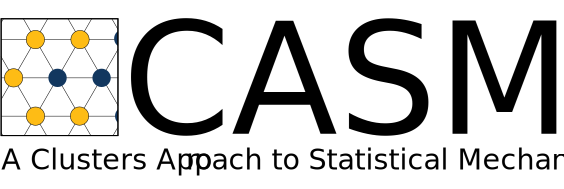
\includegraphics[height=23mm,keepaspectratio]{logo}} % Logo box - maximum height/width:
}

%----------------------------------------------------------------------------------------
%	HEADER INFORMATION
%----------------------------------------------------------------------------------------

\fancyhead[L]{\begin{tabular}{l r | l r} % The header is a table with 4 columns
\textbf{Project} & ABCD1234 & \textbf{Page} & \thepage/\pageref{LastPage} \\ % Project name and page count
\textbf{Job} & 0001 & \textbf{Updated} & 27/11/2012 \\ % Job number and last updated date
\textbf{Version} & Design-1A-RC-001 & \textbf{Reviewed} & 2/12/2012 \\ % Version and reviewed date
\textbf{Designer} & John Thomas Smith & \textbf{Reviewer} & James Smith \\ % Designer and reviewer
\end{tabular}}

%----------------------------------------------------------------------------------------

\begin{document}

\AddToShipoutPicture{\BackgroundStructure} % Set the background of each page to that specified above in the header information section

%----------------------------------------------------------------------------------------
%	DOCUMENT CONTENT
%----------------------------------------------------------------------------------------

\section{Design Check}

\marginnote{All units are \\ \textbf{[kN, mm]}}

This will need at least one design check for a general format of the equations, reference and set out.

\subsection{Preliminary Design of Members}

Will start with the same member sizes as Aurecon (for both $9$m and $10$m EBFs). Ductility, $\mu=5.75$.

\par\vspace{\baselineskip}

\begin{tabular}{|l||l|l|l|}
\hline
Member & Designation & Category & $\lambda_e$\\
\hline
Active Link & 360UB57 & 1 & 25 \\
Collector Beam & 360UB57 & 2 & 30 \\
Column & 310UC137 & 2 & 30 \\
Brace & 250UC73 & 3A & 40 \\
\hline
\end{tabular}

\par\vspace{\baselineskip}

\subsubsection{Active Links (360UB57)}

From NZS3404; link length:\marginnote{$V^*=442\mathrm{kN}$}

\begin{equation*}
\tag{Cl 5.12.1.2}
e\leqslant1.6M_s/V_v
\end{equation*}

\tab $M_s=303\mathrm{kN}$ (Capacity Tables) \\[8pt]
\tab $V_v=0.6 \times f_{yw} \times d \times t_w = 0.6 \times 320 \times 359 \times 8 = 551$kN (Cl 6.5.3) \\[8pt]
\tab $0.8$m$\leqslant0.880$m \marginnote{OK} \\

From NZS3404; link shear strength:

\begin{equation*}
\tag{Cl 6.5.3}
\phi V_v \geqslant V^*
\end{equation*}

\tab $\phi V_v=0.9\times V_v=0.9\times551=496$kN \\[8pt]
\tab $496$kN$\geqslant442$kN \marginnote{OK} \\

From NZS3404; link web slenderness:

\begin{equation}
\tag{Cl 12.8.3}
\lambda_e \leqslant \lambda_{eq}
\end{equation}

\tab $\lambda_{e1}=25$ (page 1) \\[8pt]
\tab $\lambda_e=d_1/t_w=338$mm$/8$mm$=41.6$ \\[8pt]
\tab $41.6 \nleqslant 25$ \marginnote{\textbf{NOT OK}} \\

Above doesn't pass the check, but that doesn't matter for this example.
\par\vspace{\baselineskip}

\begin{center}
\textbf{ADOPT 360UB57 FOR ALL ACTIVE LINKS} \\
\end{center}

\subsubsection{Collector Beam (360UB57)}
And so on\dots

%----------------------------------------------------------------------------------------

\end{document}
